\documentclass[11pt]{article}

\usepackage[scale=0.75,a4paper]{geometry}
\usepackage{graphicx}
\usepackage{subcaption}
\usepackage{float}
\usepackage{amsmath}
\usepackage{amssymb}
\usepackage[utf8]{inputenc}
\usepackage{lipsum}
\usepackage[british]{babel}
\usepackage{csquotes}
\usepackage[separate-uncertainty=true]{siunitx}
\usepackage[
    backend=biber,
    style=numeric,
    sorting=none
]{biblatex}

\addbibresource{references.bib}

\newcommand{\ve}[1]{\mathbf{#1}}

\begin{document}
\title{An Investigation of Phase-Locked Loops}
\author{Dan Seremet (ds780)}
\maketitle

\begin{figure}
    \centering
    \begin{subfigure}{.5\textwidth}
        \centering
        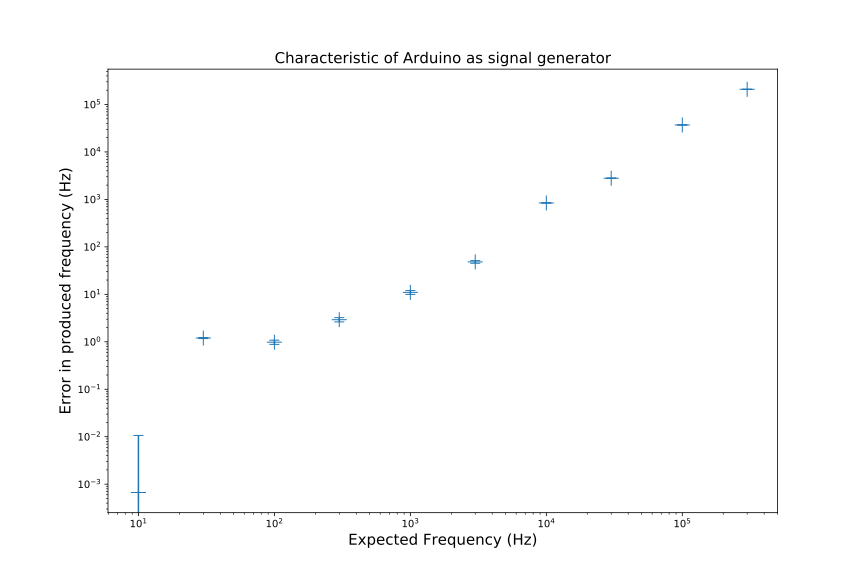
\includegraphics[width=.9\textwidth]{../docs/arduino_clever}
        \caption{Absolute errors}\label{fig:sub1}
    \end{subfigure}%
    \begin{subfigure}{.5\textwidth}
        \centering
        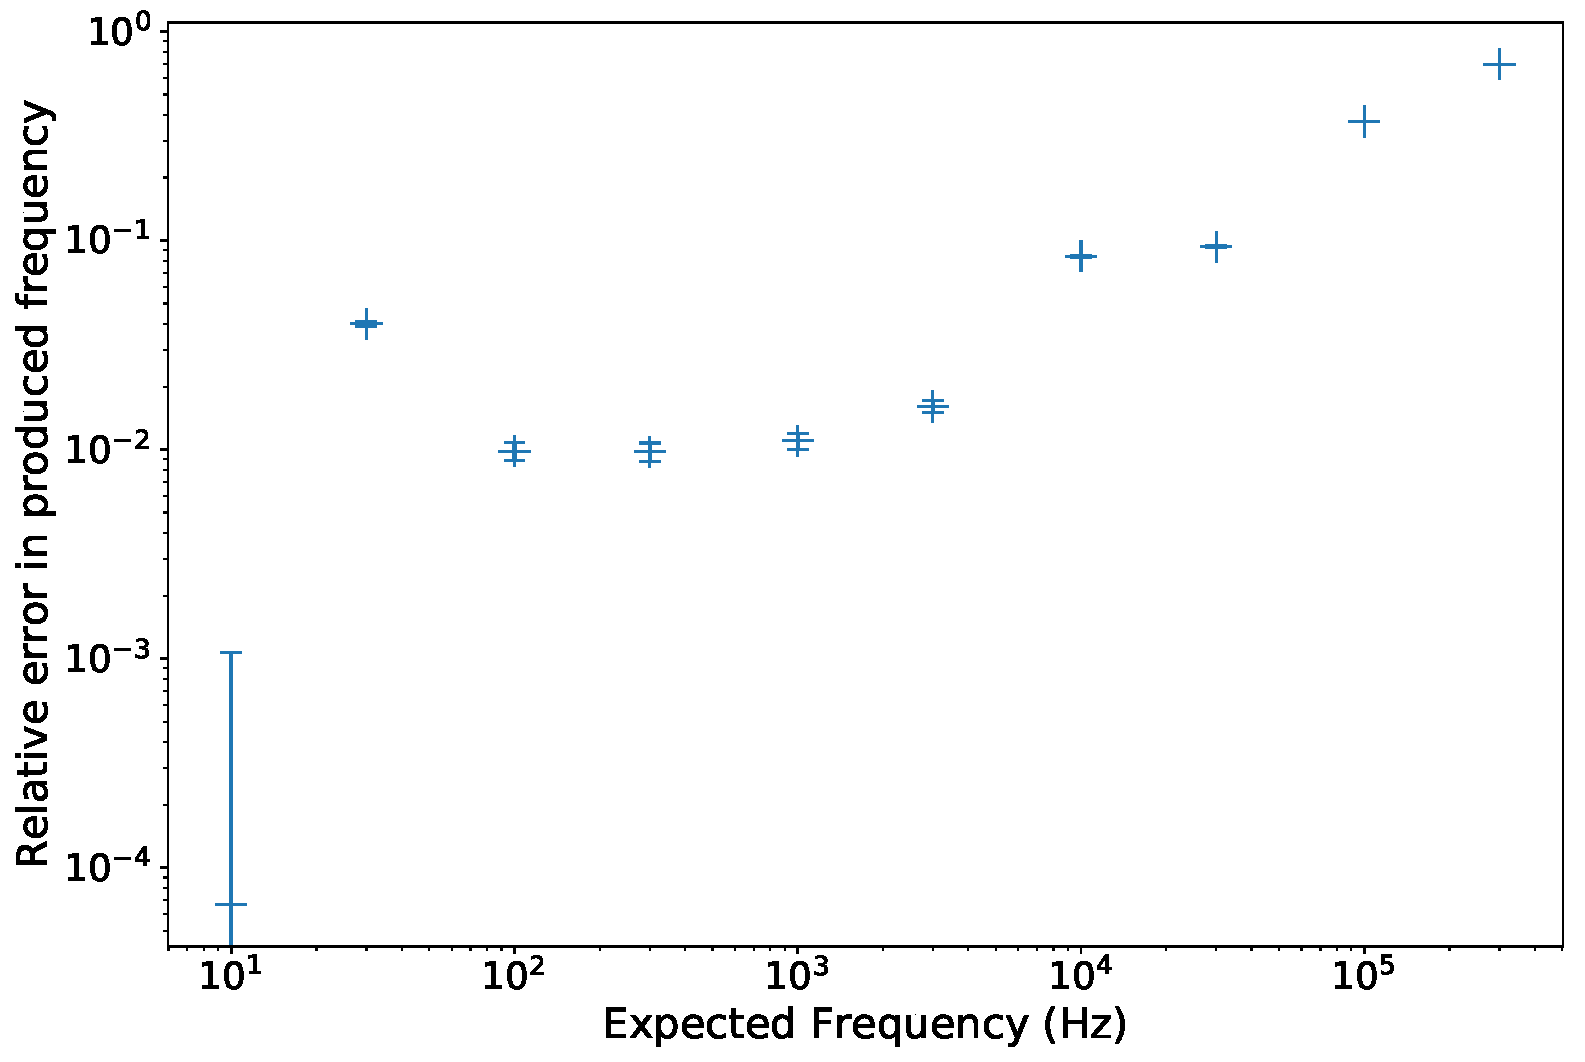
\includegraphics[width=.9\textwidth]{../docs/arduino_clever_rel}
        \caption{Relative errors}\label{fig:sub2}
    \end{subfigure}
    \caption{A figure with two subfigures}\label{fig:test}
\end{figure}
    

\end{document}